\documentclass{X:/Documents/Coding/Latex/myassignment}
\title{Topic C Assignment 5}

\begin{document}

\maketitle
\begin{enumerate}
	\item 
	\[I(x) = \int_{-\infty}^{\infty} \frac{e^{2ixt(1-t^2/6+3it/4)}}{t^2+9} dt\] 

	\begin{enumerate}
		\item Identify saddle points and paths of steepest descent/ascent through them
		

		We have $f(t) = \frac{1}{t^2+9}$ and $\phi(t) = 2it(1-t^2/6+3it/4)$.
		\[\phi(t) = i2t-it^3/3-3t^2/2\]
		Saddle when:
		\begin{align*}
			\phi'(t) = 0\\
			\implies 2i - it^2 -3t =0\\
			it^2 + 3t - 2i = 0\\
			(t-i)(it+2) =0\\
			\implies t = i,\, 2i
		\end{align*}
		Let $t = \xi + i\eta$
		\begin{align*}
			\phi(t) &=  2it(1-t^2/6+3it/4)\\
			\phi(\xi+i\eta) &= 2i(\xi+i\eta)\left(1 - (\xi+i\eta)^2/6 + 3i(\xi+i\eta)/4\right)\\
			&= -\frac{\eta^3}{3}+i\eta^2 \xi +\frac{3\eta ^2}{2}+\eta  \xi^2-i3\eta \xi - 2\eta -\frac{i\xi ^3 }{3}-\frac{3 \xi ^2}{2}+i2\xi\\
			&= -\frac{\eta ^3}{3}+\frac{3\eta ^2}{2}+\eta\xi^2-2\eta -\frac{3\xi ^2}{2}+ i\left(\eta ^2\xi -3\eta\xi -\frac{\xi ^3}{3}+2\xi\right)
		\end{align*}
		For $t=i$, $\eta = 1$, $\xi = 0$. We require the complex part to be constant on lines through this point:
		\begin{align*}
			Im(\phi) &= \eta ^2\xi -3\eta\xi -\frac{\xi ^3}{3}+2\xi\\
			Im(\phi(t=i))&=0\\					
		\end{align*}
		For $t=i2$, $\eta = 2$, $\xi = 0$
		\begin{align*}
			Im(\phi) &= \eta ^2\xi -3\eta\xi -\frac{\xi ^3}{3}+2\xi\\
			Im(\phi(t=i2))&=0\\		
		\end{align*}

		So all paths go through $Im(\phi) = 0$:
		\begin{align*}
			\implies \eta^2 \xi - 3\eta\xi - \frac{\xi^3}{3} + 2\xi &=0\\
			\eta^ 2- 3\eta - \frac{\xi^2}{3} + 2 &=0\\
			\xi = \pm\sqrt{3\eta^2 - 9\eta + 6 },\, 0\\
			\xi = \pm \sqrt{3(\eta-1)(\eta-2)}
		\end{align*}
		Noting that the zero solution is contained in the other solution.

		Identifying which is ascent and which is descent - look at the real part of $\phi$ on these paths, noting that all $\xi$ terms are $\xi^2$. 

		For the square root $\xi$:
		\begin{align*}
			Re(\phi) &= -\frac{\eta ^3}{3}+\frac{3\eta ^2}{2}+\eta\xi^2-2\eta -\frac{3\xi ^2}{2}\\
			&=-\frac{\eta^3}{3} + \frac{3\eta^2}{2} + \eta\left(3\eta^2-9\eta + 6\right) - 2\eta - \frac{3(3\eta^2-9\eta + 6)}{2}\\
			&=-\frac{\eta^3}{3} + \frac{3\eta^2}{2} + 3\eta^3-9\eta^2 + 6\eta - 2\eta - \frac{9\eta^2-27\eta + 18)}{2}\\
			&=\frac{8\eta^3}{3} - 12\eta^2 + \frac{35\eta}{2} - 9
		\end{align*}
		Which is negative for small and negative $\eta$. I.e. the descent path will be that where $\eta$ decreases (and hence $\xi$ increases). 
		And noting that the $\xi = 0$ solution gives vertical movement. 

		Direction of the path near the saddle
		\begin{align*}
			\xi &= \pm\sqrt{3\eta^2 - 9\eta + 6 }\\
			\dd{\xi}{\eta} &= \pm\frac{\left(6\eta -9\right)}{2\sqrt{\eta ^2-3\eta +2}}\\
			\dd{\xi}{\eta}\pipe_{\eta = 1} &= \pm\frac{\left(6 -9\right)}{2\sqrt{1-3 +2}} = \pm\infty\\
			\dd{\xi}{\eta}\pipe_{\eta = 2} &= \pm\frac{\left(8 -9\right)}{2\sqrt{4-6 +2}} = \pm\infty\\
		\end{align*}
		So around the saddle, the movement is strictly horizontal. It can be parameterised as 
		\[t =s + i \]


		

		% \item Plot the saddles and paths of steepest descent/ascent
		\begin{figure}[h]
			\centering
			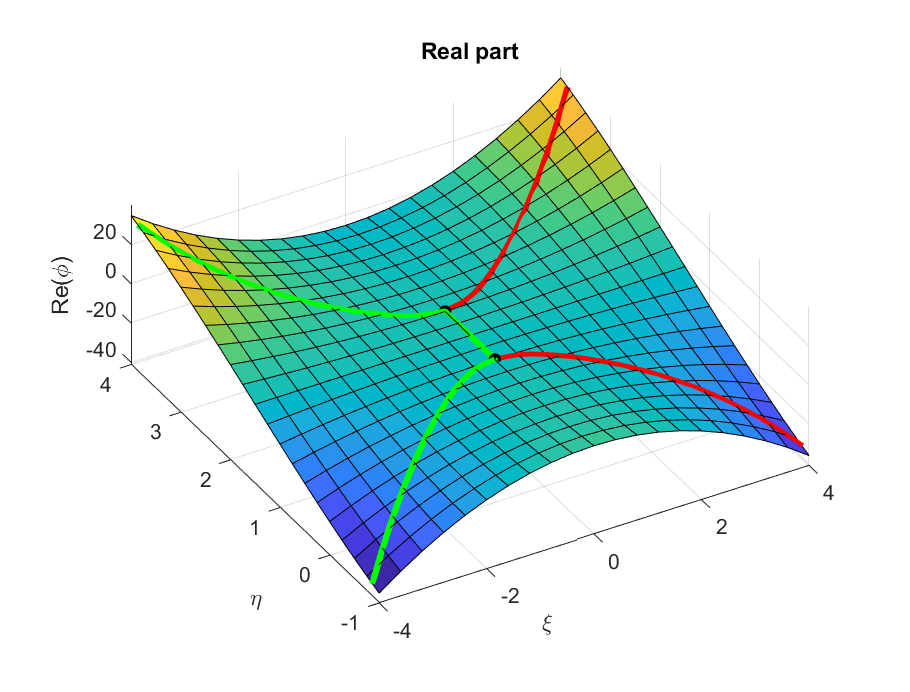
\includegraphics[width=0.8\linewidth]{TopicCA5Q1real.eps}
			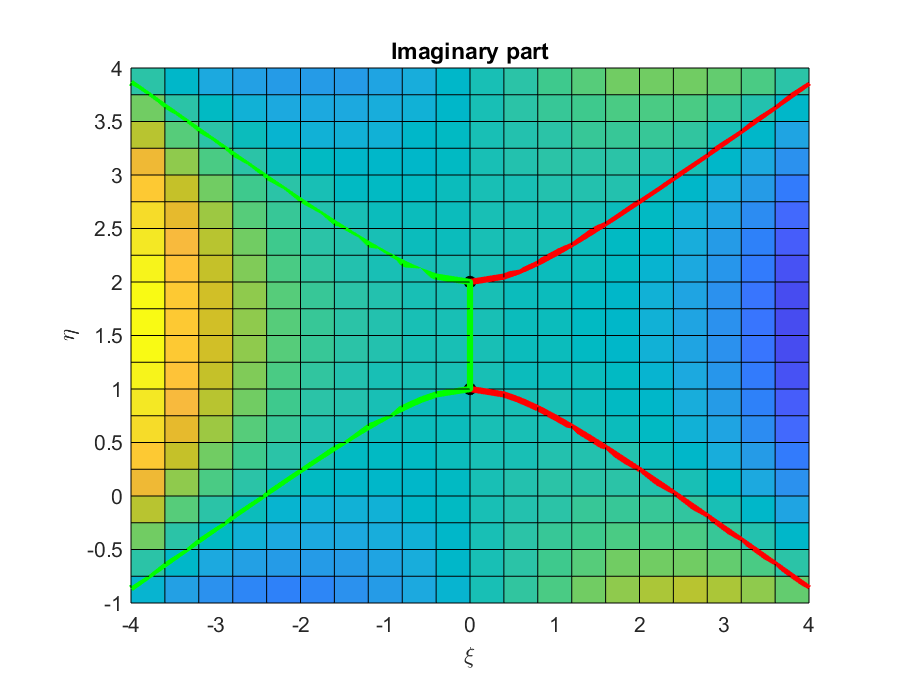
\includegraphics[width=0.8\linewidth]{TopicCA5Q1imag.eps}
			\caption{Plots of the real and imaginary parts of $\phi$, with saddles and paths of steepest descent and ascent.}
			\label{fig:q1}
		\end{figure}

		Figure~\ref{fig:q1path} plots the chosen path. Where the paths are then vertically connected to $\eta=0$ for $\xi=\pm \infty$. The assumption that this is negligible is made
		\begin{figure}[tbh]
			\centering
			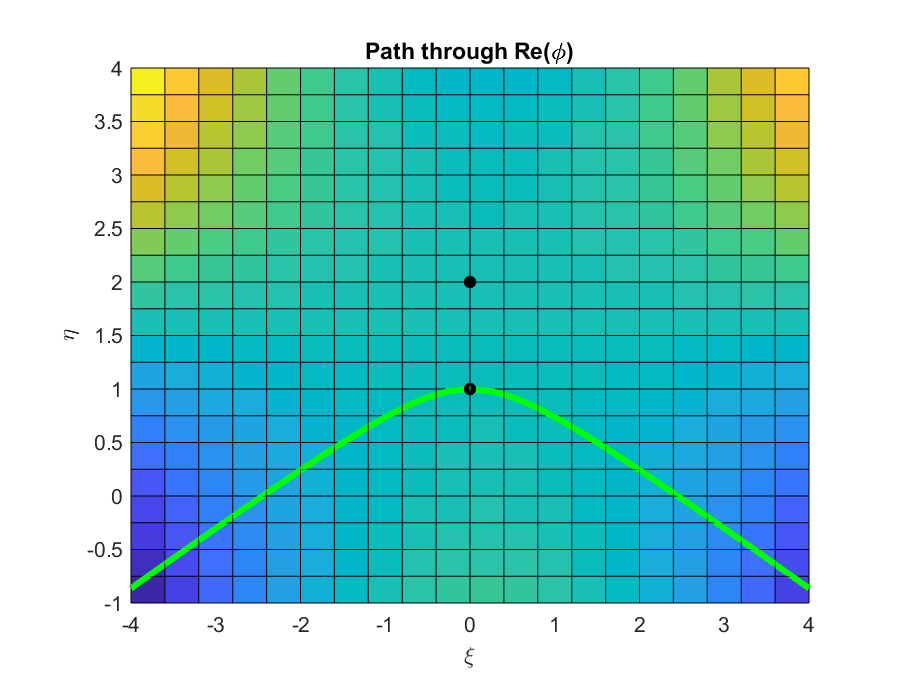
\includegraphics[width=0.8\linewidth]{TopicCA5Q1path.eps}
			\caption{Plot of the imaginary part of $\phi$, with the magenta line showing the deformed contour}
			\label{fig:q1path}
		\end{figure}

		% \item Use the deformed contour to approximate $I(x)$ to leading-order as $x\to\infty$


		Parameterise using the square root path in the integral, locally it is horizontal so $t = s+i$
		\begin{align*}
			I &= \int_{-\infty}^{\infty} \frac{e^{2ixt(1-t^2/6+3it/4)}}{t^2+9} dt\\
			\end{align*}
			Approximate the taylor series for $\frac{1}{t^2+9}$ to leading order:
		\begin{align*}
			&\sim \int_{-\infty}^{\infty} \frac{e^{2ixt(1-t^2/6+3it/4)}}{9} dt\\
			&=\frac19\int_{-\epsilon}^{\epsilon}e^{-\frac{x\left(s^32i+3s^2+5\right)}{6}} ds\\
			&=\frac{e^{-5x/6}}{9}\int_{-\epsilon}^{\epsilon}e^{-\frac{xs^2\left(2is+3\right)}{6}} ds\\
			&= \frac{e^{-5x/6}}{9}\int_{-\epsilon}^{\epsilon}e^{-\frac{xs^2\left(2is+3\right)}{6}}ds\\
			&\sim \frac{e^{-5x/6}}{9}\int_{-\epsilon}^{\epsilon}e^{-\frac{xs^2}{2}} ds\\
			&= \frac{e^{-5x/6}}{9}\int_{-\infty}^{\infty}e^{-\frac{xs^2}{2}} ds\\
			&=\frac{e^{-5x/6}}{9} \sqrt{\frac{2\pi}{x}}
		\end{align*}
		To leading order.


	\end{enumerate}
	















	\clearpage
	\item Show that
	\[I(x) = \frac12 \int_{-1}^1 e^{-4xt^2 + 5ixt - ixt^3} dt \sim \frac12 e^{-2x} \sqrt{\pi/x} ,\quad \text{ as } x\to\infty\]
	Note
	\begin{itemize}
		\item The deformed steepest descent path should have the same endpoints as the original contour
		\item The contributions from the end points are negligible compared to that from a saddle point (show this)
	\end{itemize}
	Rewrite as
	\[I(x) = \frac12 \int_{-1}^{1} e^{x\left(-4t^2+5it-it^3\right)}\]
	\[\phi(t) = -4t^2 + i5t - it^3\]
	Find any saddle points:
 
	\begin{align*}
		\phi'(t) = -8t + i5 - i3t^2 &=0 \\
		(it-1)(3t-5i)&=0\\
		t &= i,\, i5/3
	\end{align*}

	$t=\xi+i\eta$
	\begin{align*}
		\phi(t) &= -4(\xi+i\eta)^2 + i5(\xi+i\eta) - i(\xi+i\eta)^3\\
		&=-4(\xi^2 -\eta^2 +i2\xi\eta) + i5(\xi+i\eta) - i(\xi^3 +i3\xi^2\eta - 3\xi\eta^2 -i\eta^3)\\
		&=-4\xi^2 +4\eta^2 -i8\xi\eta +i5\xi -5\eta - i\xi^3 +3\xi^2\eta + i3\xi\eta^2 -\eta^3\\
		&=-4\xi^2 + 4\eta^2 - 5\eta + 3\xi^2\eta -\eta^3 + i\left(-8\xi\eta + 5\xi - \xi^3 + 3\xi\eta^2\right)
	\end{align*}


	Steepest paths for $t=0+ in$, $\xi = 0$, $\eta = n$
	\begin{align*}
		Im(\phi) &= -8\xi\eta + 5\xi - \xi^3 + 3\xi\eta^2\\
		Im(\phi(t=i))&= 0 = Im(\phi(t=i5/3))
	\end{align*}
	\begin{align*}
		-8\xi\eta + 5\xi - \xi^3 + 3\xi\eta^2 &=0\\
		-8\eta + 5 - \xi^2 +3\eta^2 &= 0\\
		\xi &= \sqrt{-8\eta + 5  +3\eta^2},\, 0\\
		\xi &= \sqrt{(3\eta - 5)(\eta - 1)},\, 0
	\end{align*}

	With local direction(s)
	\begin{align*}
		\dd{\xi}{\eta} &= \frac{6\eta-8}{2\sqrt{\left(3\eta-5\right)\left(\eta-1\right)}}\\
		\dd{\xi}{\eta}\pipe_{\eta = 1,5/3} &= \infty
	\end{align*}
	I.e. locally $t= i+s$

	Considering the end points:

	Steepest path around $t=\pm1$ so $\xi = \pm1, \eta = 0$.
	\begin{align*}
		Im(\phi) &=-8\xi\eta + 5\xi - \xi^3 + 3\xi\eta^2\\
		Im(\phi(t=\pm1))&=\pm5 \mp1 = \pm4
	\end{align*}
	For $t=-1$ want $Im(\phi) = -4$
	\begin{align*}
		-8\xi\eta + 5\xi - \xi^3 + 3\xi\eta^2 &= -4\\
		3\xi\eta^2 - 8\xi\eta -\xi^3 + 5\xi +4 &=0\\
		\eta &= \frac{8\xi \pm \sqrt{64\xi^2 - 4(3\xi)(-\xi^3 + 5\xi +4)}}{6\xi}\\
		\eta &= \frac{4\xi \pm \sqrt{\xi(16\xi +3\xi^3 - 15\xi -12))}}{6\xi}\\
		\eta &= \frac{4\xi \pm \sqrt{\xi(3\xi^3 + \xi -12)}}{3\xi}
	\end{align*}
	With direction:

	\begin{align*}
		\dd\eta\xi &= \pm\frac{\xi ^3+2}{\xi \sqrt{\xi \left(3\xi ^3+\xi -12\right)}}\\
		\dd\eta\xi\pipe_{\xi=-1} &= \pm\frac{-1+2}{-1\sqrt{-1\left(-3-1 -12\right)}} = \frac{\pm 1}{4}\\
	\end{align*}

	For $t=1$ want $Im(\phi) = 4$
	\begin{align*}
		-8\xi\eta + 5\xi - \xi^3 + 3\xi\eta^2 &= 4\\
		3\xi\eta^2 - 8\xi\eta -\xi^3 + 5\xi -4 &=0\\
		\eta &= \frac{8\xi \pm \sqrt{64\xi^2 - 4(3\xi)(-\xi^3 + 5\xi -4)}}{6\xi}\\
		\eta &= \frac{4\xi \pm \sqrt{\xi(16\xi +3\xi^3 - 15\xi +12))}}{6\xi}\\
		\eta &= \frac{4\xi \pm \sqrt{\xi(3\xi^3 + \xi +12)}}{3\xi}
	\end{align*}
	With direction:
	\begin{align*}
		\dd\eta\xi &= \pm\frac{\xi ^3-2}{\xi \sqrt{\xi \left(3\xi ^3+\xi +12\right)}}\\
		\dd\eta\xi\pipe_{\xi=1} &= \frac{\pm 1}{4}\\
	\end{align*}
	I.e. parameterise as $t =1 + s(1+\frac{i}4)$



		\begin{figure}[h]
			\centering
			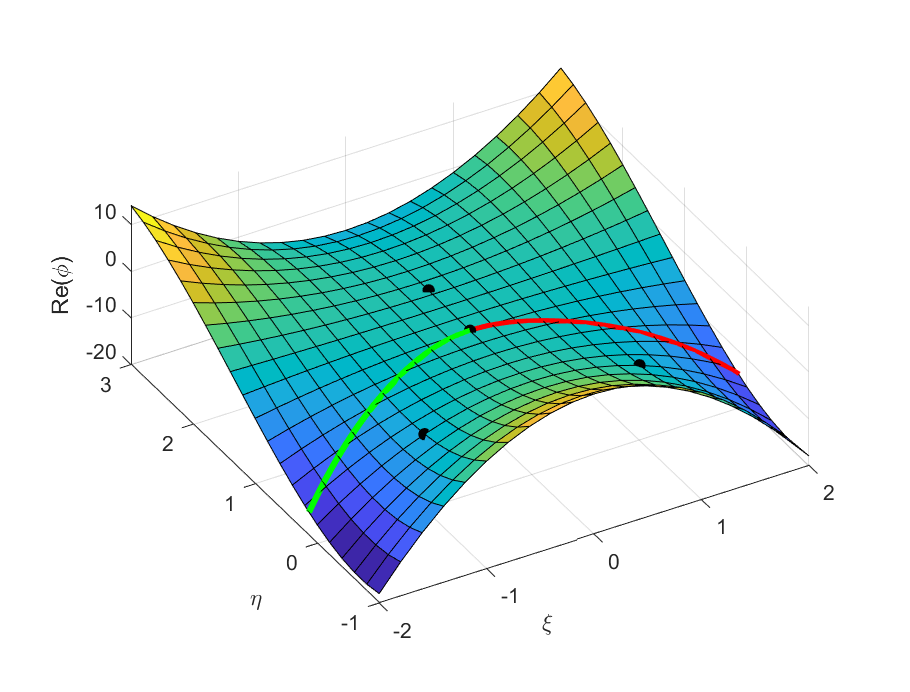
\includegraphics[width=0.8\linewidth]{TopicCA5Q2real.eps}
			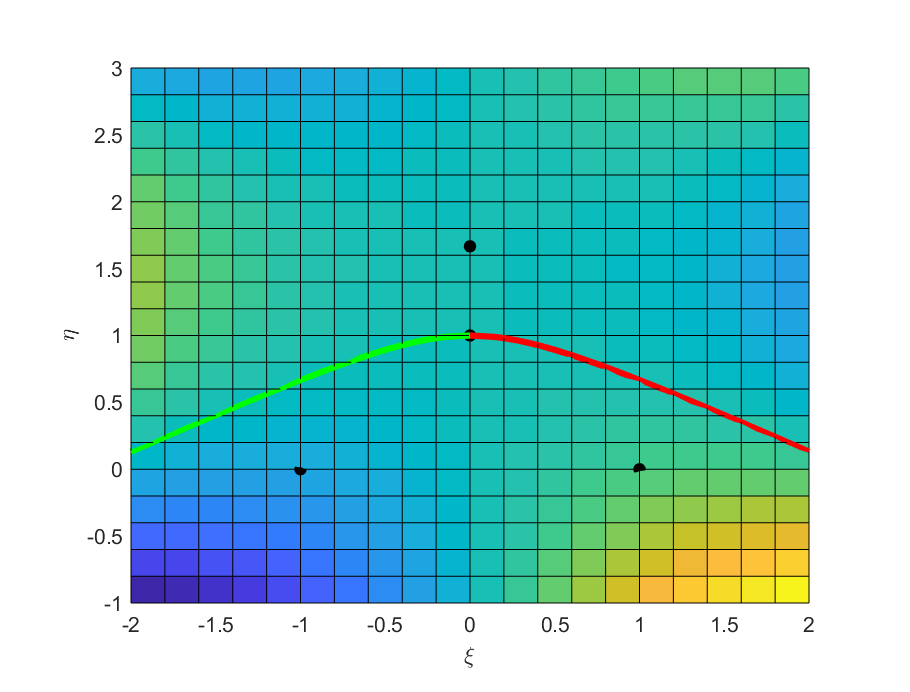
\includegraphics[width=0.8\linewidth]{TopicCA5Q2imag.eps}
			\caption{Plots of the real and imaginary parts of $\phi$, with saddles and paths of steepest descent through the chosen saddle, $\eta=1$.}
			\label{fig:q2}
		\end{figure}


	The chosen path is plotted in figure~\ref{fig:q2path}. 
	\begin{figure}[tb]
		\centering
		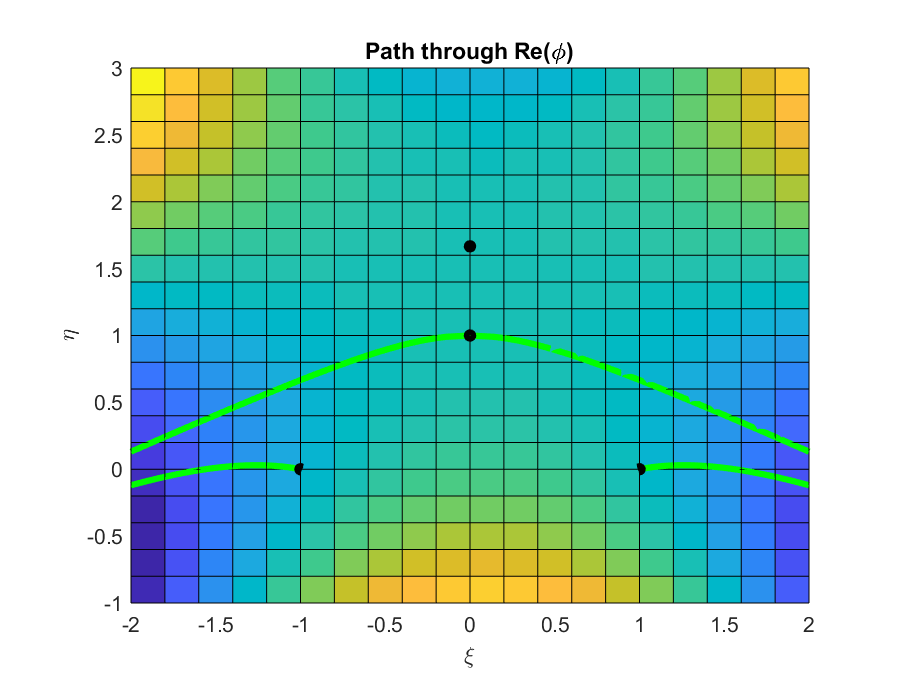
\includegraphics[width=0.8\linewidth]{TopicCA5Q2path.eps}
		\caption{Chosen path, going left from $\xi=-1$ to $\xi=-\infty$, back to $\xi=0$, through $\xi=0$ to $\xi =\infty$ then from $\xi=\infty$ to $\xi=1$}
		\label{fig:q2path}
	\end{figure}

	Path from the end point leftward:

	\begin{align*}
		I_1&=\frac12 \int_{C_1} e^{x\left(-4t^2+5it-it^3\right)}\\
		&=\frac12 \int_{C_1} e^{x\left(-4(-1 + s(1+\frac{i}4))^2+5i(-1 + s(1+\frac{i}4))-i(-1 + s(1+\frac{i}4))^3\right)} ds\\
		&=\frac12 \int_{0}^{-\infty} e^{x\left(s\left(\frac{15}{2}+4i\right)+s^2\left(-\frac{21}{4}+\frac{13}{16}i\right)+s^3\left(\frac{47}{64}-\frac{13}{16}i\right)-4-4i\right)} ds
	\end{align*}
	Noting that all of the real parts go to $0$ as $s\to -\infty$. Which is negligible, and the same occurs for the right point to $\infty$.


	Only case about local behaviour around $t=i$ so parameterise as $t = s+i$.

	\begin{align*}
		I(x) &= \frac12 \int_{-1}^{1} e^{x\left(-4t^2+5it-it^3\right)}\\
			&=\frac12 \int_{-\epsilon}^{\epsilon} e^{x\left(-4(s+i)^2+5i(s+i)-i(s+i)^3\right)}ds\\
			&= \frac12 \int_{-\epsilon}^{\epsilon} e^{x(- is^3 - s^2 - 2)}ds\\
			&= \frac12 e^{-2x} \int_{-\epsilon}^{\epsilon} e^{-x(is^3 + s^2)}ds\\
			&= \frac12 e^{-2x} \int_{-\epsilon}^{\epsilon} e^{-xs^2(is +1)}ds\\
			&\sim \frac12 e^{-2x} \int_{-\epsilon}^{\epsilon} e^{-xs^2}ds\\
			&\sim \frac12 e^{-2x} \int_{-\infty}^{\infty} e^{-xs^2}ds\\
			&\sim \frac12 e^{-2x} \sqrt{\pi/x}\\
	\end{align*}
	To leading order, as required.







\end{enumerate}

\clearpage
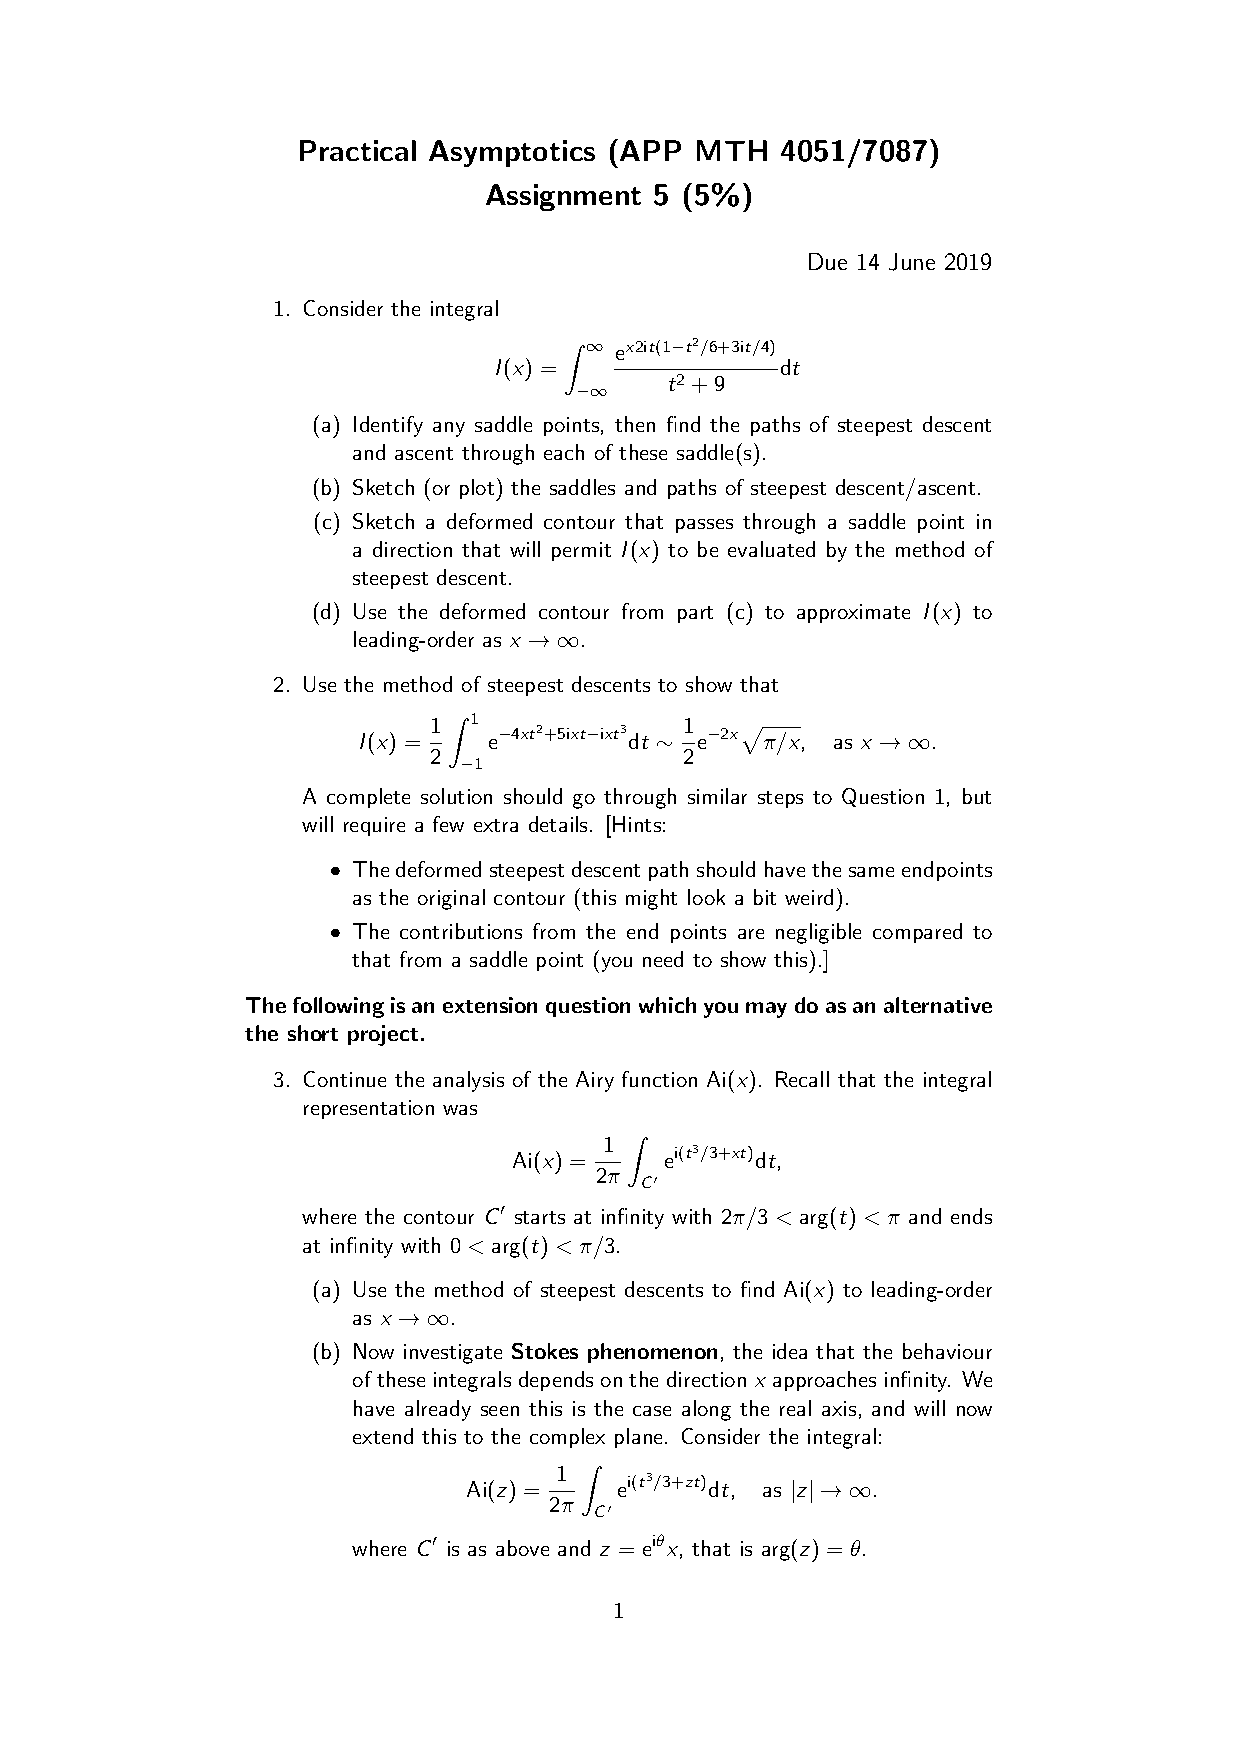
\includepdf[pages=1-]{PA_2019_A5.pdf}
\end{document}